\documentclass[14pt,a4paper]{extarticle}

\usepackage[T2A]{fontenc}
\usepackage[utf8]{inputenc}
\usepackage[english,russian]{babel}
\usepackage{tempora}
\usepackage[left=25mm,right=20mm,top=20mm,bottom=20mm]{geometry}
\usepackage{setspace}
\usepackage{indentfirst}
\usepackage{pdfpages}
\usepackage{titlesec}
\usepackage{enumitem}
\usepackage[backend=biber,style=ieee,autocite=inline]{biblatex}
\addbibresource{ref.bib}
\usepackage{hyperref}

\hypersetup{colorlinks=true, allcolors=black, urlcolor=black, linkcolor=black, citecolor=black}
\AtBeginBibliography{\hypersetup{urlcolor=black}}

\onehalfspacing
\setlength{\parindent}{1.25cm}

\titleformat*{\section}{\bfseries\centering\large}
\pagestyle{plain}

\begin{document}

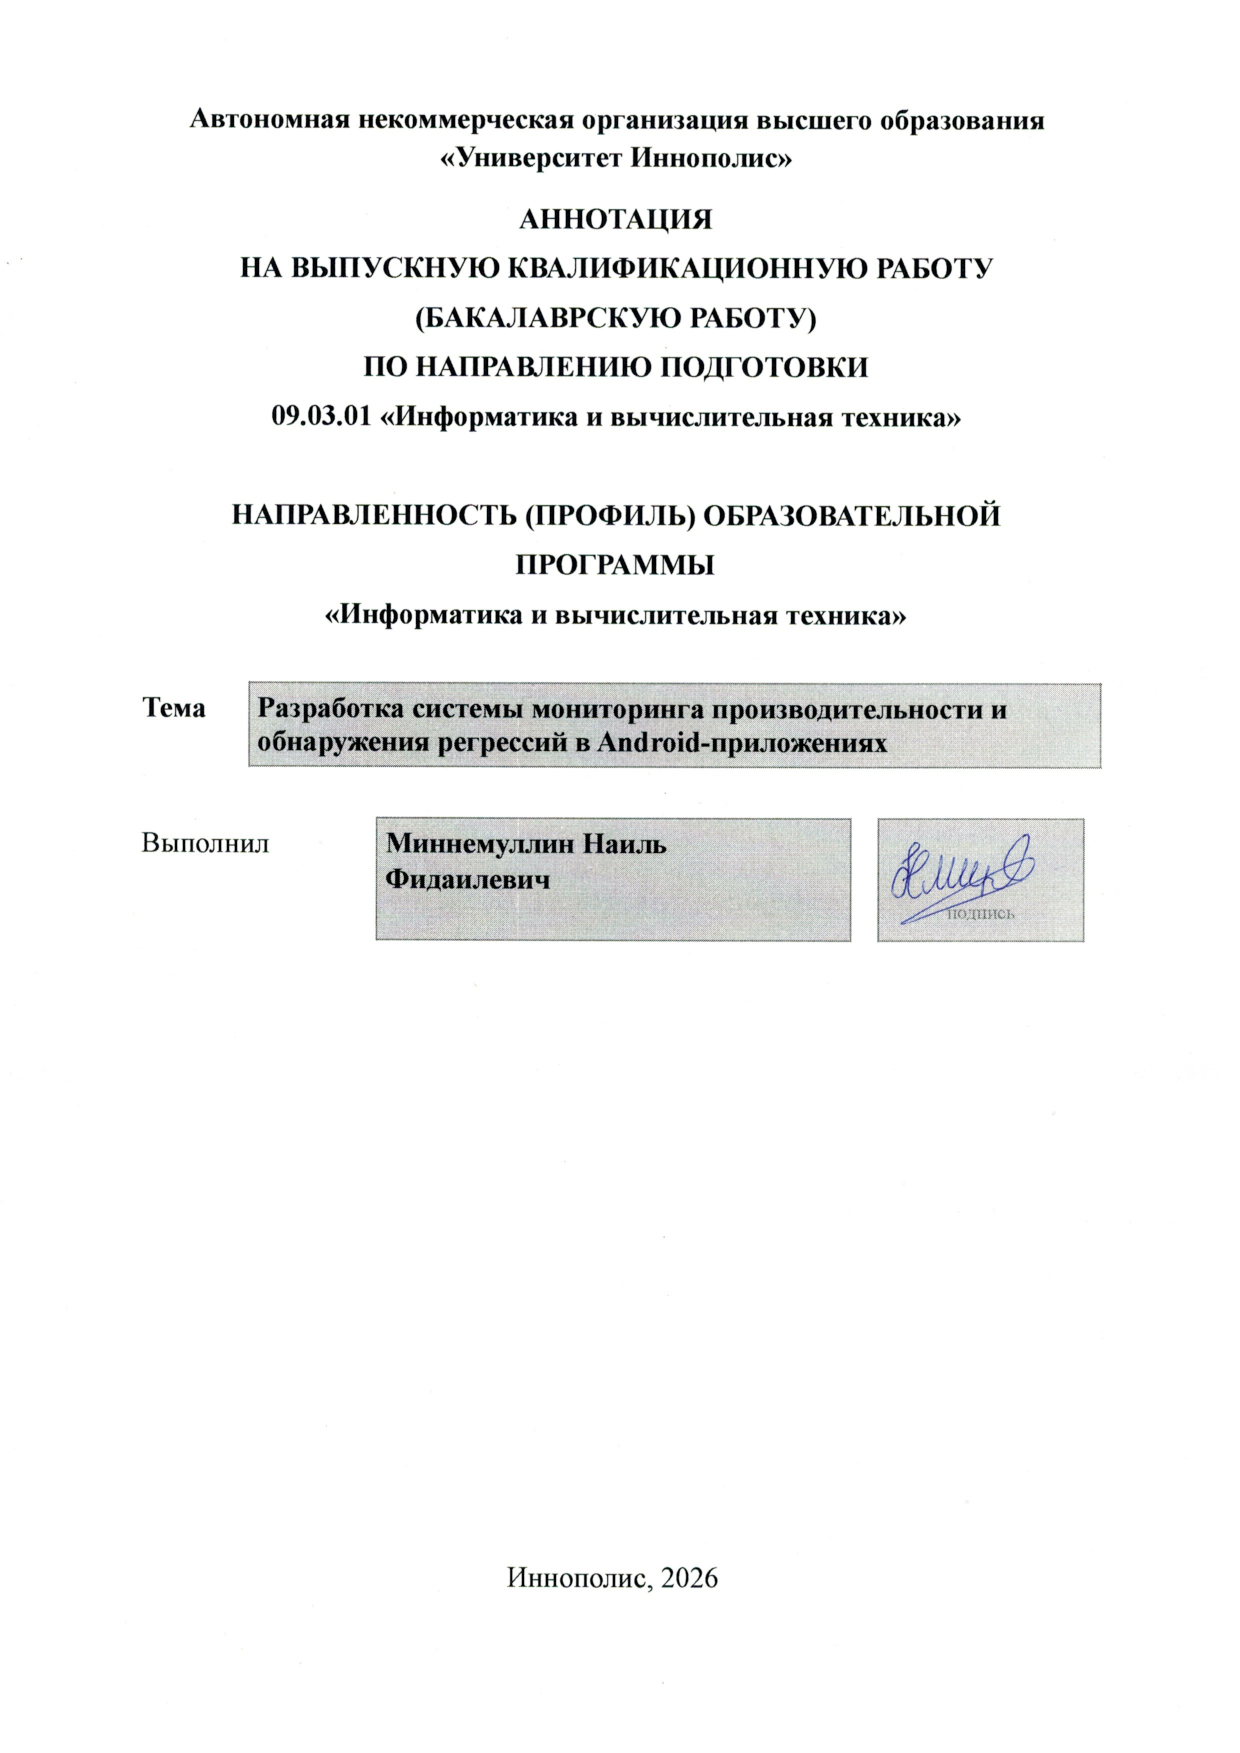
\includepdf{annotation_title.pdf}

\newpage

%% ===================== Содержание ВКР (1--2 стр.) =====================
\begin{center}
\textbf{\large Содержание выпускной квалификационной работы}
\end{center}
\vspace{0.3cm}


\begin{description}[leftmargin=0pt,labelwidth=0pt,itemindent=0pt,labelsep=0pt,style=unboxed,itemsep=0pt,parsep=0pt,font=\normalfont]

\item[\textbf{1\quad Введение}\dotfill 7]
\item[\quad 1.1\quad Предметная область и мотивация\dotfill 7]
\item[\quad 1.2\quad Исследовательский пробел\dotfill 8]
\item[\quad 1.3\quad Исследовательские вопросы и цель работы\dotfill 8]
\item[\quad 1.4\quad Новизна и вклад\dotfill 9]
\item[\quad 1.5\quad Структура работы\dotfill 10]

\item[\textbf{2\quad Обзор литературы}\dotfill 11]
\item[\quad 2.1\quad Мониторинг производительности\dotfill 12]
\item[\quad 2.2\quad Подходы к сбору данных о производительности\dotfill 12]
\item[\quad 2.3\quad Метрики производительности\dotfill 16]
\item[\quad 2.4\quad Обнаружение регрессий производительности\dotfill 17]
\item[\quad 2.5\quad Выводы\dotfill 20]

\item[\textbf{3\quad Методология}\dotfill 22]
\item[\quad 3.1\quad Требования и ограничения системы\dotfill 22]
\item[\quad 3.2\quad Высокоуровневая архитектура\dotfill 23]
\item[\quad 3.3\quad Проектирование мобильного SDK\dotfill 24]
\item[\quad 3.4\quad Проектирование backend-сервиса\dotfill 28]
\item[\quad 3.5\quad Выводы\dotfill 33]

\item[\textbf{4\quad Реализация}\dotfill 34]
\item[\quad 4.1\quad Реализация мобильного SDK\dotfill 34]
\item[\quad 4.2\quad Реализация backend-сервиса\dotfill 41]
\item[\quad 4.3\quad Реализация обнаружения регрессий\dotfill 44]
\item[\quad 4.4\quad Реализация frontend-дашборда\dotfill 46]
\item[\quad 4.5\quad Выводы\dotfill 50]

\item[\textbf{5\quad Оценка и обсуждение}\dotfill 51]
\item[\quad 5.1\quad Установка валидации\dotfill 51]
\item[\quad 5.2\quad Оценка накладных расходов SDK\dotfill 52]
\item[\quad 5.3\quad Сквозное тестирование системы\dotfill 54]
\item[\quad 5.4\quad Обсуждение результатов\dotfill 58]
\item[\quad 5.5\quad Ограничения и направления дальнейшей работы\dotfill 60]

\item[\textbf{6\quad Заключение}\dotfill 62]
\item[\textbf{Список использованной литературы}\dotfill 64]
\end{description}

\newpage

%% ===================== Введение (1 стр.) =====================
\section*{Введение}

Каждый новый релиз мобильного приложения может незаметно ухудшать производительность на разлчиных экранах, например через добавление нового фунционала или обновление внешних зависимостей. На Android такие регрессии особенно трудно выявить, поскольку устройства пользователей сильно различаются по характеристикам и версиям операционной системы, и один и тот же релиз может вести себя по-разному на разных устройствах. Автоматическое обнаружение регрессий хорошо изучено для серверных систем~\cite{Kayenta}, однако существующие инструменты для Android с поддержкой оповещений в основном опираются на пороги, задаваемые разработчиком вручную, и сравнивают все устройства вместе, не учитывая различий в их производительности~\cite{FirebasePerf}.

\textbf{Цель работы} состоит в разработке системы, которая непрерывно собирает метрики производительности с Android-устройств пользователей и автоматически обнаруживает регрессии между релизами с учётом различных классов производительности устройств. Ключевая новизна состоит в том, что релизы сравниваются не по совокупности всех устройств, а внутри отдельных когорт со схожими характеристиками. Слабые устройства обычно составляют меньшую долю собранных данных. При сравнении по всем устройствам сразу регрессия, заметная только на слабых устройствах, теряется на фоне данных с более производительных. Однако поддержание производительности на таких устройствах не менее важно~\cite{Zikan}.

\textbf{Задачи работы.} (1) Проанализировать существующие подходы к мониторингу и обнаружению регрессий на Android. (2) Спроектировать архитектуру системы из SD для Android, backend-сервиса и пользовательского интерфейса. (3) Реализовать на устройстве сбор метрик производительности с низкими накладными расходами. (4) Реализовать метод обнаружения регрессий, учитывающий различные классы устройств. (5) Экспериментально  подтвердить работоспособность системы, оценить накладные расходы SDK на устройствах и показать эффективность стратификации по когортам.

\newpage

%% ===================== Краткое описание основной части (1 стр.) =====================
\section*{Краткое описание основной части работы}

\noindent\textbf{Обзор литературы (глава 2).} Во второй главе анализируются подходы к сбору данных о производительности на Android, которые делятся на предрелизное профилирование и пострелизный мониторинг, а также методы автоматического обнаружения регрессий~\cite{Nguyen2012, FBDetect}. Рассматривается фрагментация устройств Android~\cite{Zikan} и схемы их сегментации по производительности. Выявленный пробел состоит в отсутствии автоматического релиз-парного обнаружения регрессий, стратифицированного по когортам устройств.

\noindent\textbf{Методология (глава 3).} В третьей главе формулируются требования к системе и описывается её архитектура из четырёх компонентов. Мобильный SDK на Kotlin собирает метрики UI, время холодного старта, загрузку CPU и объём используемой памяти. Backend-сервис на Ktor принимает батчи метрик, хранит реляционные данные в PostgreSQL, временные ряды в ClickHouse~\cite{schulze2024clickhouse} и относит устройства к когортам Low, Medium и High. Сервис обнаружения регрессий для каждой пары последовательных релизов вычисляет относительный сдвиг P95 в разрезе метрики, экрана и когорты и фиксирует регрессию при превышении порога в 15 процентов.

\noindent\textbf{Реализация (глава 4).} В четвёртой главе описывается реализация компонентов. SDK написан на Kotlin с буферизацией метрик в Room и пакетной передачей по сети, а backend на Ktor с авторизацией через JWT и BCrypt. Дашборд построен на Streamlit. Сервис обнаружения регрессий реализован на Python, использует агрегирующие запросы ClickHouse и отправляет уведомления в Telegram. Все компоненты упакованы в Docker и развёрнуты как открытая система.

\noindent\textbf{Оценка и обсуждение (глава 5).} В пятой главе система проверяется экспериментально. Накладные расходы SDK не превысили 5,2 процентных пункта загрузки CPU, 5,4 МБ (4,1 процента) оперативной памяти и 75 мс (5,1 процента) времени холодного старта. Тестирование системы подтвердило корректность её работы. Также разделение на когорты оказалось полезным: регрессия, проявляющаяся только на слабых устройствах, была успешно обнаружена.

\newpage

%% ===================== Заключение (1 стр.) =====================
\section*{Заключение}

Результатом работы стала спроектированная, реализованная и экспериментально проверенная система мониторинга производительности Android-приложений и автоматического обнаружения регрессий между релизами. Последовательные релизы сравниваются не по всем устройствам сразу, а независимо внутри когорт Low, Medium и High, что позволяет находить регрессии, проявляющиеся только на определённом классе устройств.

Эмпирически показано, что SDK сохраняет работоспособность при низких накладных расходах. В худшем случае на тестовых устройствах прирост загрузки CPU не превысил 5,2 процентных пункта, использования памяти 5,4 МБ (4,1 процента), а времени холодного старта 75 мс (5,1 процента). Сквозное тестирование подтвердило, что система корректно фиксирует регрессии. В эксперименте с регрессией, чувствительной к классу устройства, разделение на когорты продемонстрировало свою эффективность: регрессия, заметная только на слабых устройствах, была успешно обнаружена, тогда как при сравнении по всем устройствам сразу она бы затерялась на фоне данных с более производительных устройств.

Тем самым работа закрывает обозначенный пробел в области автоматического пострелизного обнаружения регрессий на Android и предлагает готовую к использованию систему со стратификацией сравнения релизов по когортам устройств. Перспективы дальнейшей работы включают расширение набора метрик, а также улучшение алгоритмов разделения на когорты и обнаружения регрессий.

\newpage

%% ===================== Список литературы (1 стр., 5--6 ссылок) =====================
\begin{center}
\textbf{\large Список использованных источников}
\end{center}
\vspace{0.4cm}
\nocite{FirebasePerf,Kayenta,Nguyen2012,FBDetect,Zikan,schulze2024clickhouse}
\printbibliography[heading=none]

\end{document}
